\chapter{Introduction}\label{chap:introduction}
Operating Systems play an important part of any modern computer system. The field of operating systems has gone through a growing-spurt in the last few years and will continue to grow effortlessly as computers have become prevalent in a lot of areas around us. You will find operating systems in cars, house-appliances, printers, and many other embedded devices.\\
\\
In front of you lies the course manual in which you will learn the basics of operating systems on an intuitive level. This guide consists of two parts. The manual consists of 5 sessions. Each session will cover an important subject of operating systems. The first session will explain what processes are and how you should use them. The second session will cover Threads and the third session will cover multithreading. Multithreading is an important concept when you want to increase the efficiency of the program you desire to run. The fourth section will show how you can effectively schedule threads and the last section will cover the synchronisation of threads.\\

Each session consists of several exercises. Once you have finished an exercise you have to let an assistent sign-off on this exercise in your manual before continuing to the next question. Additionally, you will have to upload your solution to CPM\footnote{http://cpm.ewi.tudelft.nl}. Here your solutions will be subjected to a plagiarism check and officially checked-off. At the end of each session you will find a programming exercise which will be more complex than the exercises you have done before in that session. However, if you manage to successfully implement/answer that question you will be rewarded with 0.2 bonus point. Therefore, if you are able to successfully answer all bonus questions, you will have 1 bonuspoint for your final exam! The bonuspoint only counts if you have all exercises checked and signed by the assistants.\\  

\section{Overview}\label{sec:overview}
Microcontrollers process instructions in a binary matter. Considering the fact that there are a lot of instructions to be called to perform a simple task, it would be time-consuming if users would execute functions by means of binary instructions. Furthermore, in order to increase the amount of users, the system must be easy to work with as not everyone has the knowledge to perform difficult instructions. An operating system acts as an intermediary between the user of a computer and the computer hardware. The purpose of an operating system is to provide an environment in which a user can execute programs in a convenient and efficient yet easy manner. An operating system disconnects the user from the hardware as the operating system is the one that translates the users' instructions to hardware instructions. Therefore, it can be seen that operating systems manage the computer hardware.\\
\\
During this lab you will be using the Raspberry Pi which is explained in further detail in section \ref{sec:raspberry} and depicted in figure \ref{fig:raspberry}.

\section{Raspberry Pi}\label{sec:raspberry}
The Raspberry Pi is a credit card-seized single-board computer created with the intention of promoting the teaching of basic computer science in schools. The Raspberry Pi is based on the Broadcomp BCM2835 system on a chip, which includes an ARM1176JZF-S 700 MHz processor, VideoCore IV GPU, and is shipped with 512 megabytes of RAM. The processor used in the Raspberry Pi is equivalent to a chip used in the early generation smartphones. The Raspberry Pi primarily uses Linux kernel-based operating systems. As mentioned in the previous section, you will be using the Raspberry Pi during this laboratory.\\
\\
\begin{figure}[!htbp]
	\centering
		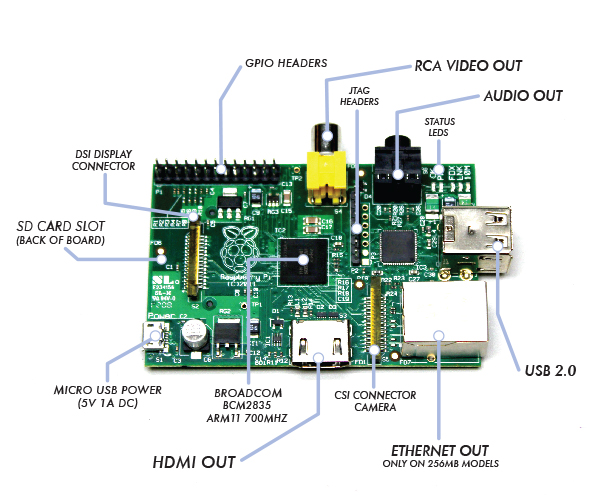
\includegraphics[width=0.80\textwidth]{images/raspberry.jpg}
	\caption{Raspberry Pi}
	\label{fig:raspberry}
\end{figure}

In the next chapter you will be guided through the installation and explained how to upload your code to the Raspberry Pi in order to test your implementation.\\ 

